
% Default to the notebook output style

    


% Inherit from the specified cell style.




    
\documentclass[11pt]{article}

    
    
    \usepackage[T1]{fontenc}
    % Nicer default font (+ math font) than Computer Modern for most use cases
    \usepackage{mathpazo}

    % Basic figure setup, for now with no caption control since it's done
    % automatically by Pandoc (which extracts ![](path) syntax from Markdown).
    \usepackage{graphicx}
    % We will generate all images so they have a width \maxwidth. This means
    % that they will get their normal width if they fit onto the page, but
    % are scaled down if they would overflow the margins.
    \makeatletter
    \def\maxwidth{\ifdim\Gin@nat@width>\linewidth\linewidth
    \else\Gin@nat@width\fi}
    \makeatother
    \let\Oldincludegraphics\includegraphics
    % Set max figure width to be 80% of text width, for now hardcoded.
    \renewcommand{\includegraphics}[1]{\Oldincludegraphics[width=.8\maxwidth]{#1}}
    % Ensure that by default, figures have no caption (until we provide a
    % proper Figure object with a Caption API and a way to capture that
    % in the conversion process - todo).
    \usepackage{caption}
    \DeclareCaptionLabelFormat{nolabel}{}
    \captionsetup{labelformat=nolabel}

    \usepackage{adjustbox} % Used to constrain images to a maximum size 
    \usepackage{xcolor} % Allow colors to be defined
    \usepackage{enumerate} % Needed for markdown enumerations to work
    \usepackage{geometry} % Used to adjust the document margins
    \usepackage{amsmath} % Equations
    \usepackage{amssymb} % Equations
    \usepackage{textcomp} % defines textquotesingle
    % Hack from http://tex.stackexchange.com/a/47451/13684:
    \AtBeginDocument{%
        \def\PYZsq{\textquotesingle}% Upright quotes in Pygmentized code
    }
    \usepackage{upquote} % Upright quotes for verbatim code
    \usepackage{eurosym} % defines \euro
    \usepackage[mathletters]{ucs} % Extended unicode (utf-8) support
    \usepackage[utf8x]{inputenc} % Allow utf-8 characters in the tex document
    \usepackage{fancyvrb} % verbatim replacement that allows latex
    \usepackage{grffile} % extends the file name processing of package graphics 
                         % to support a larger range 
    % The hyperref package gives us a pdf with properly built
    % internal navigation ('pdf bookmarks' for the table of contents,
    % internal cross-reference links, web links for URLs, etc.)
    \usepackage{hyperref}
    \usepackage{longtable} % longtable support required by pandoc >1.10
    \usepackage{booktabs}  % table support for pandoc > 1.12.2
    \usepackage[inline]{enumitem} % IRkernel/repr support (it uses the enumerate* environment)
    \usepackage[normalem]{ulem} % ulem is needed to support strikethroughs (\sout)
                                % normalem makes italics be italics, not underlines
    

    
    
    % Colors for the hyperref package
    \definecolor{urlcolor}{rgb}{0,.145,.698}
    \definecolor{linkcolor}{rgb}{.71,0.21,0.01}
    \definecolor{citecolor}{rgb}{.12,.54,.11}

    % ANSI colors
    \definecolor{ansi-black}{HTML}{3E424D}
    \definecolor{ansi-black-intense}{HTML}{282C36}
    \definecolor{ansi-red}{HTML}{E75C58}
    \definecolor{ansi-red-intense}{HTML}{B22B31}
    \definecolor{ansi-green}{HTML}{00A250}
    \definecolor{ansi-green-intense}{HTML}{007427}
    \definecolor{ansi-yellow}{HTML}{DDB62B}
    \definecolor{ansi-yellow-intense}{HTML}{B27D12}
    \definecolor{ansi-blue}{HTML}{208FFB}
    \definecolor{ansi-blue-intense}{HTML}{0065CA}
    \definecolor{ansi-magenta}{HTML}{D160C4}
    \definecolor{ansi-magenta-intense}{HTML}{A03196}
    \definecolor{ansi-cyan}{HTML}{60C6C8}
    \definecolor{ansi-cyan-intense}{HTML}{258F8F}
    \definecolor{ansi-white}{HTML}{C5C1B4}
    \definecolor{ansi-white-intense}{HTML}{A1A6B2}

    % commands and environments needed by pandoc snippets
    % extracted from the output of `pandoc -s`
    \providecommand{\tightlist}{%
      \setlength{\itemsep}{0pt}\setlength{\parskip}{0pt}}
    \DefineVerbatimEnvironment{Highlighting}{Verbatim}{commandchars=\\\{\}}
    % Add ',fontsize=\small' for more characters per line
    \newenvironment{Shaded}{}{}
    \newcommand{\KeywordTok}[1]{\textcolor[rgb]{0.00,0.44,0.13}{\textbf{{#1}}}}
    \newcommand{\DataTypeTok}[1]{\textcolor[rgb]{0.56,0.13,0.00}{{#1}}}
    \newcommand{\DecValTok}[1]{\textcolor[rgb]{0.25,0.63,0.44}{{#1}}}
    \newcommand{\BaseNTok}[1]{\textcolor[rgb]{0.25,0.63,0.44}{{#1}}}
    \newcommand{\FloatTok}[1]{\textcolor[rgb]{0.25,0.63,0.44}{{#1}}}
    \newcommand{\CharTok}[1]{\textcolor[rgb]{0.25,0.44,0.63}{{#1}}}
    \newcommand{\StringTok}[1]{\textcolor[rgb]{0.25,0.44,0.63}{{#1}}}
    \newcommand{\CommentTok}[1]{\textcolor[rgb]{0.38,0.63,0.69}{\textit{{#1}}}}
    \newcommand{\OtherTok}[1]{\textcolor[rgb]{0.00,0.44,0.13}{{#1}}}
    \newcommand{\AlertTok}[1]{\textcolor[rgb]{1.00,0.00,0.00}{\textbf{{#1}}}}
    \newcommand{\FunctionTok}[1]{\textcolor[rgb]{0.02,0.16,0.49}{{#1}}}
    \newcommand{\RegionMarkerTok}[1]{{#1}}
    \newcommand{\ErrorTok}[1]{\textcolor[rgb]{1.00,0.00,0.00}{\textbf{{#1}}}}
    \newcommand{\NormalTok}[1]{{#1}}
    
    % Additional commands for more recent versions of Pandoc
    \newcommand{\ConstantTok}[1]{\textcolor[rgb]{0.53,0.00,0.00}{{#1}}}
    \newcommand{\SpecialCharTok}[1]{\textcolor[rgb]{0.25,0.44,0.63}{{#1}}}
    \newcommand{\VerbatimStringTok}[1]{\textcolor[rgb]{0.25,0.44,0.63}{{#1}}}
    \newcommand{\SpecialStringTok}[1]{\textcolor[rgb]{0.73,0.40,0.53}{{#1}}}
    \newcommand{\ImportTok}[1]{{#1}}
    \newcommand{\DocumentationTok}[1]{\textcolor[rgb]{0.73,0.13,0.13}{\textit{{#1}}}}
    \newcommand{\AnnotationTok}[1]{\textcolor[rgb]{0.38,0.63,0.69}{\textbf{\textit{{#1}}}}}
    \newcommand{\CommentVarTok}[1]{\textcolor[rgb]{0.38,0.63,0.69}{\textbf{\textit{{#1}}}}}
    \newcommand{\VariableTok}[1]{\textcolor[rgb]{0.10,0.09,0.49}{{#1}}}
    \newcommand{\ControlFlowTok}[1]{\textcolor[rgb]{0.00,0.44,0.13}{\textbf{{#1}}}}
    \newcommand{\OperatorTok}[1]{\textcolor[rgb]{0.40,0.40,0.40}{{#1}}}
    \newcommand{\BuiltInTok}[1]{{#1}}
    \newcommand{\ExtensionTok}[1]{{#1}}
    \newcommand{\PreprocessorTok}[1]{\textcolor[rgb]{0.74,0.48,0.00}{{#1}}}
    \newcommand{\AttributeTok}[1]{\textcolor[rgb]{0.49,0.56,0.16}{{#1}}}
    \newcommand{\InformationTok}[1]{\textcolor[rgb]{0.38,0.63,0.69}{\textbf{\textit{{#1}}}}}
    \newcommand{\WarningTok}[1]{\textcolor[rgb]{0.38,0.63,0.69}{\textbf{\textit{{#1}}}}}
    
    
    % Define a nice break command that doesn't care if a line doesn't already
    % exist.
    \def\br{\hspace*{\fill} \\* }
    % Math Jax compatability definitions
    \def\gt{>}
    \def\lt{<}
    % Document parameters
    \title{Business\_Location\_Analysis}
    
    
    

    % Pygments definitions
    
\makeatletter
\def\PY@reset{\let\PY@it=\relax \let\PY@bf=\relax%
    \let\PY@ul=\relax \let\PY@tc=\relax%
    \let\PY@bc=\relax \let\PY@ff=\relax}
\def\PY@tok#1{\csname PY@tok@#1\endcsname}
\def\PY@toks#1+{\ifx\relax#1\empty\else%
    \PY@tok{#1}\expandafter\PY@toks\fi}
\def\PY@do#1{\PY@bc{\PY@tc{\PY@ul{%
    \PY@it{\PY@bf{\PY@ff{#1}}}}}}}
\def\PY#1#2{\PY@reset\PY@toks#1+\relax+\PY@do{#2}}

\expandafter\def\csname PY@tok@w\endcsname{\def\PY@tc##1{\textcolor[rgb]{0.73,0.73,0.73}{##1}}}
\expandafter\def\csname PY@tok@c\endcsname{\let\PY@it=\textit\def\PY@tc##1{\textcolor[rgb]{0.25,0.50,0.50}{##1}}}
\expandafter\def\csname PY@tok@cp\endcsname{\def\PY@tc##1{\textcolor[rgb]{0.74,0.48,0.00}{##1}}}
\expandafter\def\csname PY@tok@k\endcsname{\let\PY@bf=\textbf\def\PY@tc##1{\textcolor[rgb]{0.00,0.50,0.00}{##1}}}
\expandafter\def\csname PY@tok@kp\endcsname{\def\PY@tc##1{\textcolor[rgb]{0.00,0.50,0.00}{##1}}}
\expandafter\def\csname PY@tok@kt\endcsname{\def\PY@tc##1{\textcolor[rgb]{0.69,0.00,0.25}{##1}}}
\expandafter\def\csname PY@tok@o\endcsname{\def\PY@tc##1{\textcolor[rgb]{0.40,0.40,0.40}{##1}}}
\expandafter\def\csname PY@tok@ow\endcsname{\let\PY@bf=\textbf\def\PY@tc##1{\textcolor[rgb]{0.67,0.13,1.00}{##1}}}
\expandafter\def\csname PY@tok@nb\endcsname{\def\PY@tc##1{\textcolor[rgb]{0.00,0.50,0.00}{##1}}}
\expandafter\def\csname PY@tok@nf\endcsname{\def\PY@tc##1{\textcolor[rgb]{0.00,0.00,1.00}{##1}}}
\expandafter\def\csname PY@tok@nc\endcsname{\let\PY@bf=\textbf\def\PY@tc##1{\textcolor[rgb]{0.00,0.00,1.00}{##1}}}
\expandafter\def\csname PY@tok@nn\endcsname{\let\PY@bf=\textbf\def\PY@tc##1{\textcolor[rgb]{0.00,0.00,1.00}{##1}}}
\expandafter\def\csname PY@tok@ne\endcsname{\let\PY@bf=\textbf\def\PY@tc##1{\textcolor[rgb]{0.82,0.25,0.23}{##1}}}
\expandafter\def\csname PY@tok@nv\endcsname{\def\PY@tc##1{\textcolor[rgb]{0.10,0.09,0.49}{##1}}}
\expandafter\def\csname PY@tok@no\endcsname{\def\PY@tc##1{\textcolor[rgb]{0.53,0.00,0.00}{##1}}}
\expandafter\def\csname PY@tok@nl\endcsname{\def\PY@tc##1{\textcolor[rgb]{0.63,0.63,0.00}{##1}}}
\expandafter\def\csname PY@tok@ni\endcsname{\let\PY@bf=\textbf\def\PY@tc##1{\textcolor[rgb]{0.60,0.60,0.60}{##1}}}
\expandafter\def\csname PY@tok@na\endcsname{\def\PY@tc##1{\textcolor[rgb]{0.49,0.56,0.16}{##1}}}
\expandafter\def\csname PY@tok@nt\endcsname{\let\PY@bf=\textbf\def\PY@tc##1{\textcolor[rgb]{0.00,0.50,0.00}{##1}}}
\expandafter\def\csname PY@tok@nd\endcsname{\def\PY@tc##1{\textcolor[rgb]{0.67,0.13,1.00}{##1}}}
\expandafter\def\csname PY@tok@s\endcsname{\def\PY@tc##1{\textcolor[rgb]{0.73,0.13,0.13}{##1}}}
\expandafter\def\csname PY@tok@sd\endcsname{\let\PY@it=\textit\def\PY@tc##1{\textcolor[rgb]{0.73,0.13,0.13}{##1}}}
\expandafter\def\csname PY@tok@si\endcsname{\let\PY@bf=\textbf\def\PY@tc##1{\textcolor[rgb]{0.73,0.40,0.53}{##1}}}
\expandafter\def\csname PY@tok@se\endcsname{\let\PY@bf=\textbf\def\PY@tc##1{\textcolor[rgb]{0.73,0.40,0.13}{##1}}}
\expandafter\def\csname PY@tok@sr\endcsname{\def\PY@tc##1{\textcolor[rgb]{0.73,0.40,0.53}{##1}}}
\expandafter\def\csname PY@tok@ss\endcsname{\def\PY@tc##1{\textcolor[rgb]{0.10,0.09,0.49}{##1}}}
\expandafter\def\csname PY@tok@sx\endcsname{\def\PY@tc##1{\textcolor[rgb]{0.00,0.50,0.00}{##1}}}
\expandafter\def\csname PY@tok@m\endcsname{\def\PY@tc##1{\textcolor[rgb]{0.40,0.40,0.40}{##1}}}
\expandafter\def\csname PY@tok@gh\endcsname{\let\PY@bf=\textbf\def\PY@tc##1{\textcolor[rgb]{0.00,0.00,0.50}{##1}}}
\expandafter\def\csname PY@tok@gu\endcsname{\let\PY@bf=\textbf\def\PY@tc##1{\textcolor[rgb]{0.50,0.00,0.50}{##1}}}
\expandafter\def\csname PY@tok@gd\endcsname{\def\PY@tc##1{\textcolor[rgb]{0.63,0.00,0.00}{##1}}}
\expandafter\def\csname PY@tok@gi\endcsname{\def\PY@tc##1{\textcolor[rgb]{0.00,0.63,0.00}{##1}}}
\expandafter\def\csname PY@tok@gr\endcsname{\def\PY@tc##1{\textcolor[rgb]{1.00,0.00,0.00}{##1}}}
\expandafter\def\csname PY@tok@ge\endcsname{\let\PY@it=\textit}
\expandafter\def\csname PY@tok@gs\endcsname{\let\PY@bf=\textbf}
\expandafter\def\csname PY@tok@gp\endcsname{\let\PY@bf=\textbf\def\PY@tc##1{\textcolor[rgb]{0.00,0.00,0.50}{##1}}}
\expandafter\def\csname PY@tok@go\endcsname{\def\PY@tc##1{\textcolor[rgb]{0.53,0.53,0.53}{##1}}}
\expandafter\def\csname PY@tok@gt\endcsname{\def\PY@tc##1{\textcolor[rgb]{0.00,0.27,0.87}{##1}}}
\expandafter\def\csname PY@tok@err\endcsname{\def\PY@bc##1{\setlength{\fboxsep}{0pt}\fcolorbox[rgb]{1.00,0.00,0.00}{1,1,1}{\strut ##1}}}
\expandafter\def\csname PY@tok@kc\endcsname{\let\PY@bf=\textbf\def\PY@tc##1{\textcolor[rgb]{0.00,0.50,0.00}{##1}}}
\expandafter\def\csname PY@tok@kd\endcsname{\let\PY@bf=\textbf\def\PY@tc##1{\textcolor[rgb]{0.00,0.50,0.00}{##1}}}
\expandafter\def\csname PY@tok@kn\endcsname{\let\PY@bf=\textbf\def\PY@tc##1{\textcolor[rgb]{0.00,0.50,0.00}{##1}}}
\expandafter\def\csname PY@tok@kr\endcsname{\let\PY@bf=\textbf\def\PY@tc##1{\textcolor[rgb]{0.00,0.50,0.00}{##1}}}
\expandafter\def\csname PY@tok@bp\endcsname{\def\PY@tc##1{\textcolor[rgb]{0.00,0.50,0.00}{##1}}}
\expandafter\def\csname PY@tok@fm\endcsname{\def\PY@tc##1{\textcolor[rgb]{0.00,0.00,1.00}{##1}}}
\expandafter\def\csname PY@tok@vc\endcsname{\def\PY@tc##1{\textcolor[rgb]{0.10,0.09,0.49}{##1}}}
\expandafter\def\csname PY@tok@vg\endcsname{\def\PY@tc##1{\textcolor[rgb]{0.10,0.09,0.49}{##1}}}
\expandafter\def\csname PY@tok@vi\endcsname{\def\PY@tc##1{\textcolor[rgb]{0.10,0.09,0.49}{##1}}}
\expandafter\def\csname PY@tok@vm\endcsname{\def\PY@tc##1{\textcolor[rgb]{0.10,0.09,0.49}{##1}}}
\expandafter\def\csname PY@tok@sa\endcsname{\def\PY@tc##1{\textcolor[rgb]{0.73,0.13,0.13}{##1}}}
\expandafter\def\csname PY@tok@sb\endcsname{\def\PY@tc##1{\textcolor[rgb]{0.73,0.13,0.13}{##1}}}
\expandafter\def\csname PY@tok@sc\endcsname{\def\PY@tc##1{\textcolor[rgb]{0.73,0.13,0.13}{##1}}}
\expandafter\def\csname PY@tok@dl\endcsname{\def\PY@tc##1{\textcolor[rgb]{0.73,0.13,0.13}{##1}}}
\expandafter\def\csname PY@tok@s2\endcsname{\def\PY@tc##1{\textcolor[rgb]{0.73,0.13,0.13}{##1}}}
\expandafter\def\csname PY@tok@sh\endcsname{\def\PY@tc##1{\textcolor[rgb]{0.73,0.13,0.13}{##1}}}
\expandafter\def\csname PY@tok@s1\endcsname{\def\PY@tc##1{\textcolor[rgb]{0.73,0.13,0.13}{##1}}}
\expandafter\def\csname PY@tok@mb\endcsname{\def\PY@tc##1{\textcolor[rgb]{0.40,0.40,0.40}{##1}}}
\expandafter\def\csname PY@tok@mf\endcsname{\def\PY@tc##1{\textcolor[rgb]{0.40,0.40,0.40}{##1}}}
\expandafter\def\csname PY@tok@mh\endcsname{\def\PY@tc##1{\textcolor[rgb]{0.40,0.40,0.40}{##1}}}
\expandafter\def\csname PY@tok@mi\endcsname{\def\PY@tc##1{\textcolor[rgb]{0.40,0.40,0.40}{##1}}}
\expandafter\def\csname PY@tok@il\endcsname{\def\PY@tc##1{\textcolor[rgb]{0.40,0.40,0.40}{##1}}}
\expandafter\def\csname PY@tok@mo\endcsname{\def\PY@tc##1{\textcolor[rgb]{0.40,0.40,0.40}{##1}}}
\expandafter\def\csname PY@tok@ch\endcsname{\let\PY@it=\textit\def\PY@tc##1{\textcolor[rgb]{0.25,0.50,0.50}{##1}}}
\expandafter\def\csname PY@tok@cm\endcsname{\let\PY@it=\textit\def\PY@tc##1{\textcolor[rgb]{0.25,0.50,0.50}{##1}}}
\expandafter\def\csname PY@tok@cpf\endcsname{\let\PY@it=\textit\def\PY@tc##1{\textcolor[rgb]{0.25,0.50,0.50}{##1}}}
\expandafter\def\csname PY@tok@c1\endcsname{\let\PY@it=\textit\def\PY@tc##1{\textcolor[rgb]{0.25,0.50,0.50}{##1}}}
\expandafter\def\csname PY@tok@cs\endcsname{\let\PY@it=\textit\def\PY@tc##1{\textcolor[rgb]{0.25,0.50,0.50}{##1}}}

\def\PYZbs{\char`\\}
\def\PYZus{\char`\_}
\def\PYZob{\char`\{}
\def\PYZcb{\char`\}}
\def\PYZca{\char`\^}
\def\PYZam{\char`\&}
\def\PYZlt{\char`\<}
\def\PYZgt{\char`\>}
\def\PYZsh{\char`\#}
\def\PYZpc{\char`\%}
\def\PYZdl{\char`\$}
\def\PYZhy{\char`\-}
\def\PYZsq{\char`\'}
\def\PYZdq{\char`\"}
\def\PYZti{\char`\~}
% for compatibility with earlier versions
\def\PYZat{@}
\def\PYZlb{[}
\def\PYZrb{]}
\makeatother


    % Exact colors from NB
    \definecolor{incolor}{rgb}{0.0, 0.0, 0.5}
    \definecolor{outcolor}{rgb}{0.545, 0.0, 0.0}



    
    % Prevent overflowing lines due to hard-to-break entities
    \sloppy 
    % Setup hyperref package
    \hypersetup{
      breaklinks=true,  % so long urls are correctly broken across lines
      colorlinks=true,
      urlcolor=urlcolor,
      linkcolor=linkcolor,
      citecolor=citecolor,
      }
    % Slightly bigger margins than the latex defaults
    
    \geometry{verbose,tmargin=1in,bmargin=1in,lmargin=1in,rmargin=1in}
    
    

    \begin{document}
    
    
    \maketitle
    
    

    
    \section{Business Location Analysis}\label{business-location-analysis}

    first drafted on 2016-07-11

last updated on 2018-06-19

\emph{by Park, Pablo Chanwoo}

    \emph{It is a critical question to many business where to open and
operate its offline spaces. Especially when a business is pursuing an
expansion to places not so familiar to, researching and making a
decision on where to locate can be a very difficult problem. I have had
a similar concerns as a strategist, and came up with a simple
alternative that helped me to make reasonable data-driven decision
making.}

    The logic is simple;

 ~~~~\emph{'You want to do business from where your customers are.'}

 In order to find such a location, the following procedure has been
taken from this analysis:

\begin{enumerate}
\def\labelenumi{\arabic{enumi}.}
\tightlist
\item
  Define customers - Define sets of customers, which the business is
  targeting to. The purpose of business, marketing, and strategy all
  come in to play. If appripriate, apply STP to each set of customer.
\item
  Define sets - For each heterogeneous set of customers, allocation of
  brand or landmark that can represent characteristics of the set. It
  can be popular brand(shop), public places, or anything that can be
  searched on google map. More specific, the better.
\item
  Find on google - Google web API provides geocode for your search
  query. Geocode for each keyword location can be retrieved.
\item
  Plot on map - Now that each location information is given, plot
  heatmap layer on google map with the help of package 'gmaps'. It can
  be done separately by each set of customers, or as a whole.
\end{enumerate}

\begin{itemize}
\tightlist
\item
  please refer to
  https://developers.google.com/maps/documentation/javascript/places?hl=ko\#place\_searches
  for more information on Google place API \_\_\_ For example, \emph{a
  restaurant franchise seeking an international expansion} into London,
  UK may take the following procedure:
\end{itemize}

\begin{enumerate}
\def\labelenumi{\arabic{enumi}.}
\tightlist
\item
  Define customers
\end{enumerate}

\begin{itemize}
\tightlist
\item
  Curious customers seeking for new things to try with fellows, with
  mid-upper range income to spare on dinning experience.
\end{itemize}

\begin{enumerate}
\def\labelenumi{\arabic{enumi}.}
\setcounter{enumi}{1}
\tightlist
\item
  Define sets
\end{enumerate}

\begin{itemize}
\tightlist
\item
  Restaurant(restaurant)
\item
  Pioneers (university, waterstones, starbucks)
\item
  Tourist (hotel, tourist attraction)
\item
  Hang out (cinema, club)
\end{itemize}

\begin{enumerate}
\def\labelenumi{\arabic{enumi}.}
\setcounter{enumi}{2}
\tightlist
\item
  Find on google
\item
  plot on map \_\_\_
\end{enumerate}

    The libraries used for this project are as follows;

\begin{itemize}
\item
  \emph{re} for pattern \& string process
\item
  \emph{gmaps} for Google maps API
\item
  \emph{urllib} for Google API and data crawling
\end{itemize}

    \begin{Verbatim}[commandchars=\\\{\}]
{\color{incolor}In [{\color{incolor}10}]:} \PY{k+kn}{from} \PY{n+nn}{urllib}\PY{n+nn}{.}\PY{n+nn}{request} \PY{k}{import} \PY{n}{urlopen}
         \PY{k+kn}{import} \PY{n+nn}{gmaps}
         \PY{k+kn}{import} \PY{n+nn}{re}
\end{Verbatim}


    \begin{itemize}
\tightlist
\item
  Define target city and retrieve geocode using google api.
\end{itemize}

    \begin{Verbatim}[commandchars=\\\{\}]
{\color{incolor}In [{\color{incolor}4}]:} \PY{n}{city} \PY{o}{=} \PY{l+s+s1}{\PYZsq{}}\PY{l+s+s1}{London}\PY{l+s+s1}{\PYZsq{}}
        
        \PY{n}{city\PYZus{}url} \PY{o}{=} \PY{l+s+s1}{\PYZsq{}}\PY{l+s+s1}{https://maps.googleapis.com/maps/api/geocode/json?address=}\PY{l+s+s1}{\PYZsq{}}
        \PY{n}{key} \PY{o}{=} \PY{l+s+s2}{\PYZdq{}}\PY{l+s+s2}{YOUR KEY HERE}\PY{l+s+s2}{\PYZdq{}}
\end{Verbatim}


    \begin{Verbatim}[commandchars=\\\{\}]
{\color{incolor}In [{\color{incolor}5}]:} \PY{n}{url} \PY{o}{=} \PY{n}{urlopen}\PY{p}{(}\PY{n}{city\PYZus{}url}\PY{o}{+}\PY{n}{city}\PY{o}{+}\PY{n}{key}\PY{p}{)}
        \PY{n}{tmp} \PY{o}{=} \PY{n}{url}\PY{o}{.}\PY{n}{readlines}\PY{p}{(}\PY{p}{)}
        \PY{k}{for} \PY{n}{i} \PY{o+ow}{in} \PY{n+nb}{range}\PY{p}{(}\PY{n+nb}{len}\PY{p}{(}\PY{n}{tmp}\PY{p}{)}\PY{p}{)}\PY{p}{:}
            \PY{k}{if} \PY{l+s+s1}{\PYZsq{}}\PY{l+s+s1}{\PYZdq{}}\PY{l+s+s1}{location}\PY{l+s+s1}{\PYZdq{}}\PY{l+s+s1}{\PYZsq{}} \PY{o+ow}{in} \PY{n+nb}{str}\PY{p}{(}\PY{n}{tmp}\PY{p}{[}\PY{n}{i}\PY{p}{]}\PY{p}{)}\PY{p}{:}
                \PY{n}{city\PYZus{}coord} \PY{o}{=}\PY{p}{(}\PY{n+nb}{float}\PY{p}{(}\PY{n}{re}\PY{o}{.}\PY{n}{sub}\PY{p}{(}\PY{l+s+s1}{\PYZsq{}}\PY{l+s+s1}{[a\PYZhy{}z}\PY{l+s+s1}{\PYZbs{}}\PY{l+s+s1}{ }\PY{l+s+s1}{\PYZdq{}}\PY{l+s+s1}{:}\PY{l+s+se}{\PYZbs{}\PYZsq{}}\PY{l+s+s1}{,}\PY{l+s+se}{\PYZbs{}\PYZbs{}}\PY{l+s+s1}{\PYZbs{}}\PY{l+s+s1}{]*}\PY{l+s+s1}{\PYZsq{}}\PY{p}{,}\PY{l+s+s1}{\PYZsq{}}\PY{l+s+s1}{\PYZsq{}}\PY{p}{,}\PY{n+nb}{str}\PY{p}{(}\PY{n}{tmp}\PY{p}{[}\PY{n}{i}\PY{o}{+}\PY{l+m+mi}{1}\PY{p}{]}\PY{p}{)}\PY{p}{)}\PY{p}{)}\PY{p}{,} \PY{n+nb}{float}\PY{p}{(}\PY{n}{re}\PY{o}{.}\PY{n}{sub}\PY{p}{(}\PY{l+s+s1}{\PYZsq{}}\PY{l+s+s1}{[a\PYZhy{}z}\PY{l+s+s1}{\PYZbs{}}\PY{l+s+s1}{ }\PY{l+s+s1}{\PYZdq{}}\PY{l+s+s1}{:}\PY{l+s+se}{\PYZbs{}\PYZsq{}}\PY{l+s+s1}{,}\PY{l+s+se}{\PYZbs{}\PYZbs{}}\PY{l+s+s1}{\PYZbs{}}\PY{l+s+s1}{]*}\PY{l+s+s1}{\PYZsq{}}\PY{p}{,}\PY{l+s+s1}{\PYZsq{}}\PY{l+s+s1}{\PYZsq{}}\PY{p}{,}\PY{n+nb}{str}\PY{p}{(}\PY{n}{tmp}\PY{p}{[}\PY{n}{i}\PY{o}{+}\PY{l+m+mi}{2}\PY{p}{]}\PY{p}{)}\PY{p}{)}\PY{p}{)}\PY{p}{)}
        \PY{n+nb}{str}\PY{p}{(}\PY{n}{city\PYZus{}coord}\PY{p}{)}\PY{p}{[}\PY{l+m+mi}{1}\PY{p}{:}\PY{o}{\PYZhy{}}\PY{l+m+mi}{1}\PY{p}{]}
\end{Verbatim}


\begin{Verbatim}[commandchars=\\\{\}]
{\color{outcolor}Out[{\color{outcolor}5}]:} '51.5073509, -0.1277583'
\end{Verbatim}
            
    \begin{itemize}
\tightlist
\item
  If you look into the data retrieved, it contains a number of location
  informations as follows;
\end{itemize}

    \begin{Verbatim}[commandchars=\\\{\}]
{\color{incolor}In [{\color{incolor}11}]:} \PY{n}{tmp}
\end{Verbatim}


\begin{Verbatim}[commandchars=\\\{\}]
{\color{outcolor}Out[{\color{outcolor}11}]:} [b'\{\textbackslash{}n',
          b'   "results" : [\textbackslash{}n',
          b'      \{\textbackslash{}n',
          b'         "address\_components" : [\textbackslash{}n',
          b'            \{\textbackslash{}n',
          b'               "long\_name" : "London",\textbackslash{}n',
          b'               "short\_name" : "London",\textbackslash{}n',
          b'               "types" : [ "locality", "political" ]\textbackslash{}n',
          b'            \},\textbackslash{}n',
          b'            \{\textbackslash{}n',
          b'               "long\_name" : "London",\textbackslash{}n',
          b'               "short\_name" : "London",\textbackslash{}n',
          b'               "types" : [ "postal\_town" ]\textbackslash{}n',
          b'            \},\textbackslash{}n',
          b'            \{\textbackslash{}n',
          b'               "long\_name" : "Greater London",\textbackslash{}n',
          b'               "short\_name" : "Greater London",\textbackslash{}n',
          b'               "types" : [ "administrative\_area\_level\_2", "political" ]\textbackslash{}n',
          b'            \},\textbackslash{}n',
          b'            \{\textbackslash{}n',
          b'               "long\_name" : "England",\textbackslash{}n',
          b'               "short\_name" : "England",\textbackslash{}n',
          b'               "types" : [ "administrative\_area\_level\_1", "political" ]\textbackslash{}n',
          b'            \},\textbackslash{}n',
          b'            \{\textbackslash{}n',
          b'               "long\_name" : "United Kingdom",\textbackslash{}n',
          b'               "short\_name" : "GB",\textbackslash{}n',
          b'               "types" : [ "country", "political" ]\textbackslash{}n',
          b'            \}\textbackslash{}n',
          b'         ],\textbackslash{}n',
          b'         "formatted\_address" : "London, UK",\textbackslash{}n',
          b'         "geometry" : \{\textbackslash{}n',
          b'            "bounds" : \{\textbackslash{}n',
          b'               "northeast" : \{\textbackslash{}n',
          b'                  "lat" : 51.6723432,\textbackslash{}n',
          b'                  "lng" : 0.148271\textbackslash{}n',
          b'               \},\textbackslash{}n',
          b'               "southwest" : \{\textbackslash{}n',
          b'                  "lat" : 51.38494009999999,\textbackslash{}n',
          b'                  "lng" : -0.3514683\textbackslash{}n',
          b'               \}\textbackslash{}n',
          b'            \},\textbackslash{}n',
          b'            "location" : \{\textbackslash{}n',
          b'               "lat" : 51.5073509,\textbackslash{}n',
          b'               "lng" : -0.1277583\textbackslash{}n',
          b'            \},\textbackslash{}n',
          b'            "location\_type" : "APPROXIMATE",\textbackslash{}n',
          b'            "viewport" : \{\textbackslash{}n',
          b'               "northeast" : \{\textbackslash{}n',
          b'                  "lat" : 51.6723432,\textbackslash{}n',
          b'                  "lng" : 0.148271\textbackslash{}n',
          b'               \},\textbackslash{}n',
          b'               "southwest" : \{\textbackslash{}n',
          b'                  "lat" : 51.38494009999999,\textbackslash{}n',
          b'                  "lng" : -0.3514683\textbackslash{}n',
          b'               \}\textbackslash{}n',
          b'            \}\textbackslash{}n',
          b'         \},\textbackslash{}n',
          b'         "place\_id" : "ChIJdd4hrwug2EcRmSrV3Vo6llI",\textbackslash{}n',
          b'         "types" : [ "locality", "political" ]\textbackslash{}n',
          b'      \}\textbackslash{}n',
          b'   ],\textbackslash{}n',
          b'   "status" : "OK"\textbackslash{}n',
          b'\}\textbackslash{}n']
\end{Verbatim}
            
    \begin{center}\rule{0.5\linewidth}{\linethickness}\end{center}

    \begin{itemize}
\tightlist
\item
  Repeat the similar procedure for customer sets, within 15km radius of
  the destination, London for instance. Store coordinates too will be
  stored in the list.
\end{itemize}

    \begin{Verbatim}[commandchars=\\\{\}]
{\color{incolor}In [{\color{incolor}29}]:} \PY{n}{restaurant} \PY{o}{=} \PY{p}{\PYZob{}}\PY{p}{\PYZcb{}}
         \PY{n}{pioneer} \PY{o}{=} \PY{p}{\PYZob{}}\PY{p}{\PYZcb{}}
         \PY{n}{tourist} \PY{o}{=} \PY{p}{\PYZob{}}\PY{p}{\PYZcb{}}
         \PY{n}{hang\PYZus{}out} \PY{o}{=} \PY{p}{\PYZob{}}\PY{p}{\PYZcb{}}
\end{Verbatim}


    \begin{Verbatim}[commandchars=\\\{\}]
{\color{incolor}In [{\color{incolor}30}]:} \PY{n}{restaurant}\PY{p}{[}\PY{l+s+s1}{\PYZsq{}}\PY{l+s+s1}{key}\PY{l+s+s1}{\PYZsq{}}\PY{p}{]} \PY{o}{=} \PY{p}{[}\PY{l+s+s1}{\PYZsq{}}\PY{l+s+s1}{restaurant}\PY{l+s+s1}{\PYZsq{}}\PY{p}{]}
         \PY{n}{pioneer}\PY{p}{[}\PY{l+s+s1}{\PYZsq{}}\PY{l+s+s1}{key}\PY{l+s+s1}{\PYZsq{}}\PY{p}{]} \PY{o}{=} \PY{p}{[}\PY{l+s+s1}{\PYZsq{}}\PY{l+s+s1}{university}\PY{l+s+s1}{\PYZsq{}}\PY{p}{,} \PY{l+s+s1}{\PYZsq{}}\PY{l+s+s1}{waterstones}\PY{l+s+s1}{\PYZsq{}}\PY{p}{,} \PY{l+s+s1}{\PYZsq{}}\PY{l+s+s1}{starbucks}\PY{l+s+s1}{\PYZsq{}}\PY{p}{]}
         \PY{n}{tourist}\PY{p}{[}\PY{l+s+s1}{\PYZsq{}}\PY{l+s+s1}{key}\PY{l+s+s1}{\PYZsq{}}\PY{p}{]} \PY{o}{=} \PY{p}{[}\PY{l+s+s1}{\PYZsq{}}\PY{l+s+s1}{hotel}\PY{l+s+s1}{\PYZsq{}}\PY{p}{,} \PY{l+s+s1}{\PYZsq{}}\PY{l+s+s1}{attraction}\PY{l+s+s1}{\PYZsq{}}\PY{p}{]}
         \PY{n}{hang\PYZus{}out}\PY{p}{[}\PY{l+s+s1}{\PYZsq{}}\PY{l+s+s1}{key}\PY{l+s+s1}{\PYZsq{}}\PY{p}{]} \PY{o}{=} \PY{p}{[}\PY{l+s+s1}{\PYZsq{}}\PY{l+s+s1}{cinema}\PY{l+s+s1}{\PYZsq{}}\PY{p}{,} \PY{l+s+s1}{\PYZsq{}}\PY{l+s+s1}{club}\PY{l+s+s1}{\PYZsq{}}\PY{p}{]}
\end{Verbatim}


    \begin{Verbatim}[commandchars=\\\{\}]
{\color{incolor}In [{\color{incolor}32}]:} \PY{n}{search\PYZus{}url} \PY{o}{=} \PY{l+s+s1}{\PYZsq{}}\PY{l+s+s1}{https://maps.googleapis.com/maps/api/place/radarsearch/json?location=}\PY{l+s+s1}{\PYZsq{}}
         \PY{n}{search\PYZus{}range} \PY{o}{=} \PY{l+s+s1}{\PYZsq{}}\PY{l+s+s1}{\PYZam{}radius=15000\PYZam{}name=}\PY{l+s+s1}{\PYZsq{}} \PY{c+c1}{\PYZsh{}radius in metre up to 50,000m}
\end{Verbatim}


    \begin{Verbatim}[commandchars=\\\{\}]
{\color{incolor}In [{\color{incolor}33}]:} \PY{k}{def} \PY{n+nf}{search}\PY{p}{(}\PY{n}{target}\PY{p}{)}\PY{p}{:}
             \PY{n}{loc} \PY{o}{=} \PY{p}{[}\PY{p}{]}
             \PY{k}{for} \PY{n}{i} \PY{o+ow}{in} \PY{n+nb}{range}\PY{p}{(}\PY{n+nb}{len}\PY{p}{(}\PY{n}{target}\PY{p}{[}\PY{l+s+s1}{\PYZsq{}}\PY{l+s+s1}{key}\PY{l+s+s1}{\PYZsq{}}\PY{p}{]}\PY{p}{)}\PY{p}{)}\PY{p}{:}
                 \PY{n}{url} \PY{o}{=} \PY{p}{(}\PY{n}{search\PYZus{}url}\PY{o}{+}\PY{n+nb}{str}\PY{p}{(}\PY{n}{city\PYZus{}coord}\PY{p}{)}\PY{p}{[}\PY{l+m+mi}{1}\PY{p}{:}\PY{o}{\PYZhy{}}\PY{l+m+mi}{1}\PY{p}{]}\PY{o}{+}\PY{n}{search\PYZus{}range}\PY{o}{+}\PY{n}{target}\PY{p}{[}\PY{l+s+s1}{\PYZsq{}}\PY{l+s+s1}{key}\PY{l+s+s1}{\PYZsq{}}\PY{p}{]}\PY{p}{[}\PY{n}{i}\PY{p}{]}\PY{o}{+}\PY{n}{key}\PY{p}{)}\PY{o}{.}\PY{n}{replace}\PY{p}{(}\PY{l+s+s1}{\PYZsq{}}\PY{l+s+s1}{ }\PY{l+s+s1}{\PYZsq{}}\PY{p}{,}\PY{l+s+s1}{\PYZsq{}}\PY{l+s+s1}{\PYZsq{}}\PY{p}{)}
                 \PY{n}{tmp} \PY{o}{=} \PY{n}{urlopen}\PY{p}{(}\PY{n}{url}\PY{p}{)}\PY{o}{.}\PY{n}{readlines}\PY{p}{(}\PY{p}{)}
             \PY{k}{for} \PY{n}{k} \PY{o+ow}{in} \PY{n+nb}{range}\PY{p}{(}\PY{n+nb}{len}\PY{p}{(}\PY{n}{tmp}\PY{p}{)}\PY{p}{)}\PY{p}{:}
                 \PY{k}{if} \PY{l+s+s1}{\PYZsq{}}\PY{l+s+s1}{location}\PY{l+s+s1}{\PYZsq{}} \PY{o+ow}{in} \PY{n+nb}{str}\PY{p}{(}\PY{n}{tmp}\PY{p}{[}\PY{n}{k}\PY{p}{]}\PY{p}{)}\PY{p}{:}
                     \PY{n}{coordinate} \PY{o}{=} \PY{p}{(}\PY{n+nb}{float}\PY{p}{(}\PY{n}{re}\PY{o}{.}\PY{n}{sub}\PY{p}{(}\PY{l+s+s1}{\PYZsq{}}\PY{l+s+s1}{[a\PYZhy{}z}\PY{l+s+s1}{\PYZbs{}}\PY{l+s+s1}{:}\PY{l+s+se}{\PYZbs{}\PYZbs{}}\PY{l+s+s1}{\PYZbs{}}\PY{l+s+s1}{,}\PY{l+s+se}{\PYZbs{}\PYZsq{}}\PY{l+s+s1}{\PYZdq{}}\PY{l+s+s1}{ ]}\PY{l+s+s1}{\PYZsq{}}\PY{p}{,}\PY{l+s+s1}{\PYZsq{}}\PY{l+s+s1}{\PYZsq{}}\PY{p}{,}\PY{n+nb}{str}\PY{p}{(}\PY{n}{tmp}\PY{p}{[}\PY{n}{k}\PY{o}{+}\PY{l+m+mi}{1}\PY{p}{]}\PY{p}{)}\PY{p}{)}\PY{p}{)}\PY{p}{)}\PY{p}{,} \PY{p}{(}\PY{n+nb}{float}\PY{p}{(}\PY{n}{re}\PY{o}{.}\PY{n}{sub}\PY{p}{(}\PY{l+s+s1}{\PYZsq{}}\PY{l+s+s1}{[a\PYZhy{}z}\PY{l+s+s1}{\PYZbs{}}\PY{l+s+s1}{:}\PY{l+s+se}{\PYZbs{}\PYZbs{}}\PY{l+s+s1}{\PYZbs{}}\PY{l+s+s1}{,}\PY{l+s+se}{\PYZbs{}\PYZsq{}}\PY{l+s+s1}{\PYZdq{}}\PY{l+s+s1}{ ]}\PY{l+s+s1}{\PYZsq{}}\PY{p}{,}\PY{l+s+s1}{\PYZsq{}}\PY{l+s+s1}{\PYZsq{}}\PY{p}{,}\PY{n+nb}{str}\PY{p}{(}\PY{n}{tmp}\PY{p}{[}\PY{n}{k}\PY{o}{+}\PY{l+m+mi}{2}\PY{p}{]}\PY{p}{)}\PY{p}{)}\PY{p}{)}\PY{p}{)}
                     \PY{n}{loc}\PY{o}{.}\PY{n}{append}\PY{p}{(}\PY{n}{coordinate}\PY{p}{)}
             \PY{n}{target}\PY{p}{[}\PY{l+s+s1}{\PYZsq{}}\PY{l+s+s1}{loc}\PY{l+s+s1}{\PYZsq{}}\PY{p}{]} \PY{o}{=} \PY{n}{loc}
\end{Verbatim}


    \begin{Verbatim}[commandchars=\\\{\}]
{\color{incolor}In [{\color{incolor}36}]:} \PY{n}{search}\PY{p}{(}\PY{n}{restaurant}\PY{p}{)}
         \PY{n}{search}\PY{p}{(}\PY{n}{pioneer}\PY{p}{)}
         \PY{n}{search}\PY{p}{(}\PY{n}{tourist}\PY{p}{)}
         \PY{n}{search}\PY{p}{(}\PY{n}{hang\PYZus{}out}\PY{p}{)}
\end{Verbatim}


    \begin{itemize}
\item
  The below sample code for gmaps returns google map with a heat map
  layer over it, using the location information retrieved.
\item
  Please note that \textbf{'gmaps' works on Jupyter Notebook }
\end{itemize}

    \begin{Verbatim}[commandchars=\\\{\}]
{\color{incolor}In [{\color{incolor}51}]:} \PY{n}{gmaps}\PY{o}{.}\PY{n}{configure}\PY{p}{(}\PY{n}{api\PYZus{}key}\PY{o}{=}\PY{n}{key}\PY{p}{)}
         
         \PY{k}{def} \PY{n+nf}{vmap}\PY{p}{(}\PY{n}{target}\PY{p}{,} \PY{n}{method} \PY{o}{=} \PY{l+m+mi}{0}\PY{p}{,} \PY{n}{point} \PY{o}{=} \PY{l+m+mi}{15}\PY{p}{)}\PY{p}{:}
                 \PY{n}{plain\PYZus{}map} \PY{o}{=} \PY{n}{gmaps}\PY{o}{.}\PY{n}{figure}\PY{p}{(}\PY{n}{center} \PY{o}{=} \PY{n}{city\PYZus{}coord}\PY{p}{,} \PY{n}{zoom\PYZus{}level} \PY{o}{=} \PY{l+m+mi}{12}\PY{p}{)}
                 \PY{k}{if} \PY{n}{method} \PY{o}{==} \PY{l+m+mi}{0}\PY{p}{:}
                     \PY{k}{try}\PY{p}{:}
                         \PY{n}{map\PYZus{}layer} \PY{o}{=} \PY{n}{gmaps}\PY{o}{.}\PY{n}{heatmap\PYZus{}layer}\PY{p}{(}\PY{n}{target}\PY{p}{[}\PY{l+s+s1}{\PYZsq{}}\PY{l+s+s1}{loc}\PY{l+s+s1}{\PYZsq{}}\PY{p}{]}\PY{p}{,} \PY{n}{point\PYZus{}radius} \PY{o}{=} \PY{n}{point}\PY{p}{)}
                     \PY{k}{except}\PY{p}{:}
                         \PY{n}{map\PYZus{}layer} \PY{o}{=} \PY{n}{gmaps}\PY{o}{.}\PY{n}{heatmap\PYZus{}layer}\PY{p}{(}\PY{n}{target}\PY{p}{,} \PY{n}{point\PYZus{}radius} \PY{o}{=} \PY{n}{point}\PY{p}{)}
                 \PY{k}{elif} \PY{n}{method} \PY{o}{==} \PY{l+m+mi}{1}\PY{p}{:}
                     \PY{k}{try}\PY{p}{:}
                         \PY{n}{map\PYZus{}layer} \PY{o}{=} \PY{n}{gmaps}\PY{o}{.}\PY{n}{symbol\PYZus{}layer}\PY{p}{(}\PY{n}{target}\PY{p}{[}\PY{l+s+s1}{\PYZsq{}}\PY{l+s+s1}{loc}\PY{l+s+s1}{\PYZsq{}}\PY{p}{]}\PY{p}{,} \PY{n}{fill\PYZus{}color} \PY{o}{=} \PY{l+s+s1}{\PYZsq{}}\PY{l+s+s1}{green}\PY{l+s+s1}{\PYZsq{}}\PY{p}{,} \PY{n}{stroke\PYZus{}color} \PY{o}{=} \PY{l+s+s1}{\PYZsq{}}\PY{l+s+s1}{green}\PY{l+s+s1}{\PYZsq{}}\PY{p}{,} \PY{n}{scale} \PY{o}{=} \PY{n+nb}{int}\PY{p}{(}\PY{n}{point}\PY{o}{/}\PY{l+m+mi}{15}\PY{o}{*}\PY{l+m+mi}{2}\PY{p}{)}\PY{p}{)}
                     \PY{k}{except}\PY{p}{:}
                         \PY{n}{map\PYZus{}layer} \PY{o}{=} \PY{n}{gmaps}\PY{o}{.}\PY{n}{symbol\PYZus{}layer}\PY{p}{(}\PY{n}{target}\PY{p}{,} \PY{n}{fill\PYZus{}color} \PY{o}{=} \PY{l+s+s1}{\PYZsq{}}\PY{l+s+s1}{green}\PY{l+s+s1}{\PYZsq{}}\PY{p}{,} \PY{n}{stroke\PYZus{}color} \PY{o}{=} \PY{l+s+s1}{\PYZsq{}}\PY{l+s+s1}{green}\PY{l+s+s1}{\PYZsq{}}\PY{p}{,} \PY{n}{scale} \PY{o}{=} \PY{n+nb}{int}\PY{p}{(}\PY{n}{point}\PY{o}{/}\PY{l+m+mi}{15}\PY{o}{*}\PY{l+m+mi}{2}\PY{p}{)}\PY{p}{)}
                 \PY{n}{plain\PYZus{}map}\PY{o}{.}\PY{n}{add\PYZus{}layer}\PY{p}{(}\PY{n}{map\PYZus{}layer}\PY{p}{)}
                 
                 \PY{k}{return} \PY{n}{plain\PYZus{}map}        
\end{Verbatim}


    \begin{Verbatim}[commandchars=\\\{\}]
{\color{incolor}In [{\color{incolor}47}]:} \PY{n}{vmap}\PY{p}{(}\PY{n}{restaurant}\PY{p}{)}
\end{Verbatim}


    
    \begin{verbatim}
Figure(layout=FigureLayout(height='420px'))
    \end{verbatim}

    
    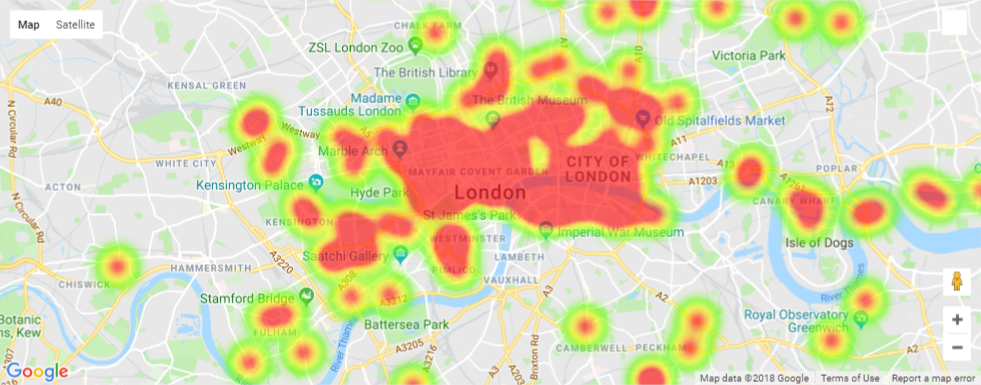
\includegraphics{restaurant_map.png} static version of gmaps output

    \begin{Verbatim}[commandchars=\\\{\}]
{\color{incolor}In [{\color{incolor}48}]:} \PY{n}{vmap}\PY{p}{(}\PY{n}{pioneer}\PY{p}{)}
\end{Verbatim}


    
    \begin{verbatim}
Figure(layout=FigureLayout(height='420px'))
    \end{verbatim}

    
    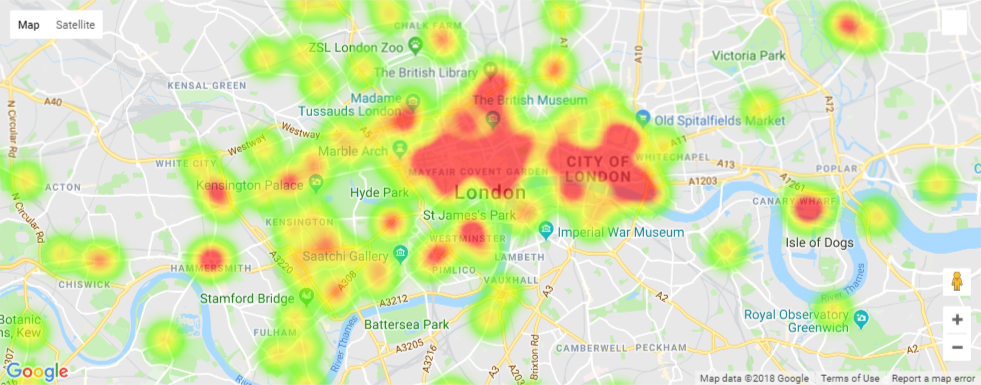
\includegraphics{pioneer_map.png} static version of gmaps output

    \begin{Verbatim}[commandchars=\\\{\}]
{\color{incolor}In [{\color{incolor}49}]:} \PY{n}{vmap}\PY{p}{(}\PY{n}{tourist}\PY{p}{)}
\end{Verbatim}


    
    \begin{verbatim}
Figure(layout=FigureLayout(height='420px'))
    \end{verbatim}

    
    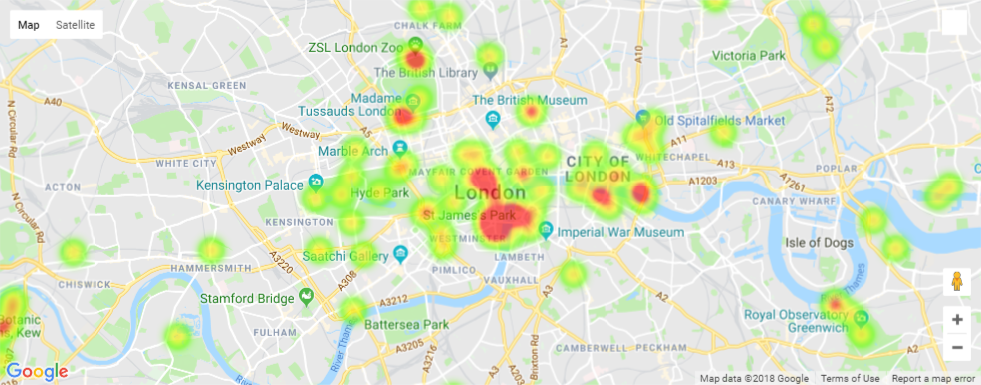
\includegraphics{tourist_map.png} static version of gmaps output

    \begin{Verbatim}[commandchars=\\\{\}]
{\color{incolor}In [{\color{incolor}52}]:} \PY{n}{vmap}\PY{p}{(}\PY{n}{hang\PYZus{}out}\PY{p}{)}
\end{Verbatim}


    
    \begin{verbatim}
Figure(layout=FigureLayout(height='420px'))
    \end{verbatim}

    
    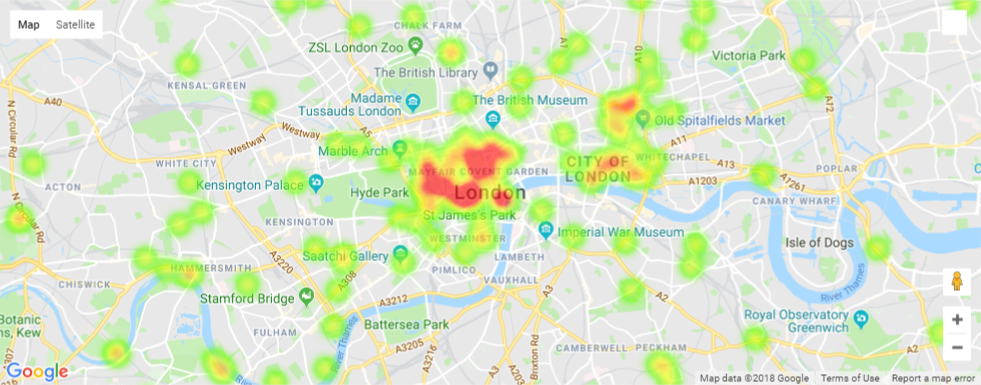
\includegraphics{hang_out_map.png} static version of gmaps output

    \begin{Verbatim}[commandchars=\\\{\}]
{\color{incolor}In [{\color{incolor}54}]:} \PY{n}{overall\PYZus{}loc} \PY{o}{=} \PY{n}{restaurant}\PY{p}{[}\PY{l+s+s1}{\PYZsq{}}\PY{l+s+s1}{loc}\PY{l+s+s1}{\PYZsq{}}\PY{p}{]} \PY{o}{+} \PY{n}{pioneer}\PY{p}{[}\PY{l+s+s1}{\PYZsq{}}\PY{l+s+s1}{loc}\PY{l+s+s1}{\PYZsq{}}\PY{p}{]} \PY{o}{+} \PY{n}{tourist}\PY{p}{[}\PY{l+s+s1}{\PYZsq{}}\PY{l+s+s1}{loc}\PY{l+s+s1}{\PYZsq{}}\PY{p}{]} \PY{o}{+} \PY{n}{hang\PYZus{}out}\PY{p}{[}\PY{l+s+s1}{\PYZsq{}}\PY{l+s+s1}{loc}\PY{l+s+s1}{\PYZsq{}}\PY{p}{]}
         \PY{n}{vmap}\PY{p}{(}\PY{n}{overall\PYZus{}loc}\PY{p}{)}
\end{Verbatim}


    
    \begin{verbatim}
Figure(layout=FigureLayout(height='420px'))
    \end{verbatim}

    
    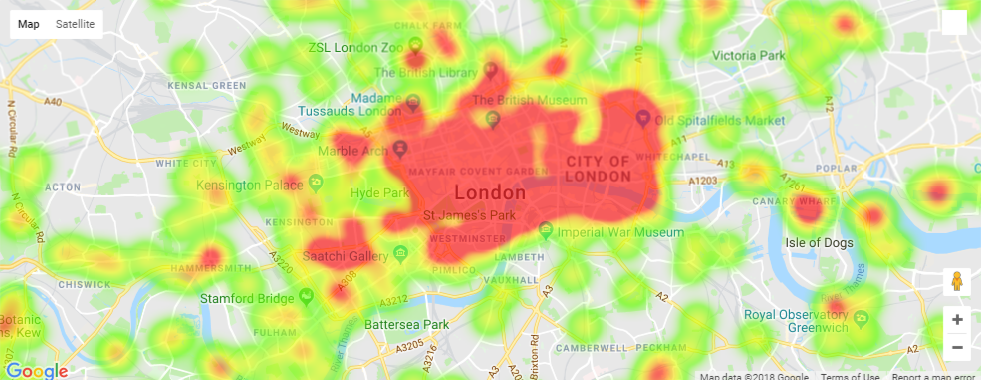
\includegraphics{overall_map.png} static version of gmaps output

    In sum, I could suggest following locations for business expansion; 1.
Kensington Place 2. XOYO 3. Bank(City of London) 4. South of London
Bridge 5. Marylebone - Covent Garden - Piccadilly Circus


    % Add a bibliography block to the postdoc
    
    
    
    \end{document}
